\newpage
\section{Conformational Fluctuations of the Rotaxane}

Having gained insight into the entropic interactions between the DNA and the
nanopore, now the stable intermediate states of the nanopiston's operation cycle are
studied. Both the rotaxane-ss and -ds are composed of stiff dsDNA and flexible ssDNA
parts, which characterise their conformational fluctuations by the entropic interactions.
The two rotaxanes types are simulated in a nanopore, using the predefined coarse-grained
model, in absence of an external bias, i.e.  $0\ mV$. The results are presented in Figure
...

Analysing the conformational fluctuations of the rotaxane-ds, we observe that the ssDNA
toehold remains predominantly outside of the pore. This effect can be explained by taking
into account the entropic cost of capturing the flexible strand of ssDNA into the
constriction of the pore. Since the geometry of the rotaxane prohibits the toehold from
reaching the cis-side of the pore, the toehold can only freely fluctuate on the
trans-side of the pore. Throughout the simulation this entropic force keeps the toehold
in the trans-reservoir and thereby placing the cis-protein stopper close to the entrance
of the pore. This entropic interaction plays an important role in the operation of the
nanopiston. Even when an external voltage difference applies an upward force on the
rotaxane, the competing entropic force keeps the toehold outside of the constriction and
thereby exposing it for hybridisation with a fuel strand. This also explains the halting
of the piston cycle at high voltages. In this case the entropic force is overcome by the
electrophoretic force induced by the voltage, sequestering the toehold inside of the pore
inhibiting the binding of fuel strands.

In the same figure the results for the rotaxane-ss are presented. The high flexibility
of the long ssDNA strand induces an entropic force upward, since this maximises the
number of configurational microstates available to the rotaxane. The flexibility of the
ssDNA strand overcomes the entropic penalty of confining the dsDNA into the constriction
of the pore. The capturing of the rotaxane-ss interface inside of the pore promotes the
operation cycle, since a longer ssDNA strand is exposed to the cis-reservoir facilitating
cargo capture. This can be seen in the positional histogram of the cis-protein stopper,
where the large fluctuations of the ssDNA strand allow it to venture far away from the
nanopore.

These results explain the functional importance of the entropic interactions in the
nanopiston's operating cycle. Comparing our findings with the results by Bayoumi et al.,
we see that both models are in reasonable accordance. However, in our simulations the
interface of the rotaxane-ss is observed entering inside the pore's constriction, while
in the spring-and-bead model this behaviour is not observed. This difference can be
attributed to the more accurate simulating of ssDNA by OxDNA, mainly arising from the
more precise parametrisation of the model and the ability for consecutive bases to
unstack.

\begin{figure}[ht!]
\begin{center}
  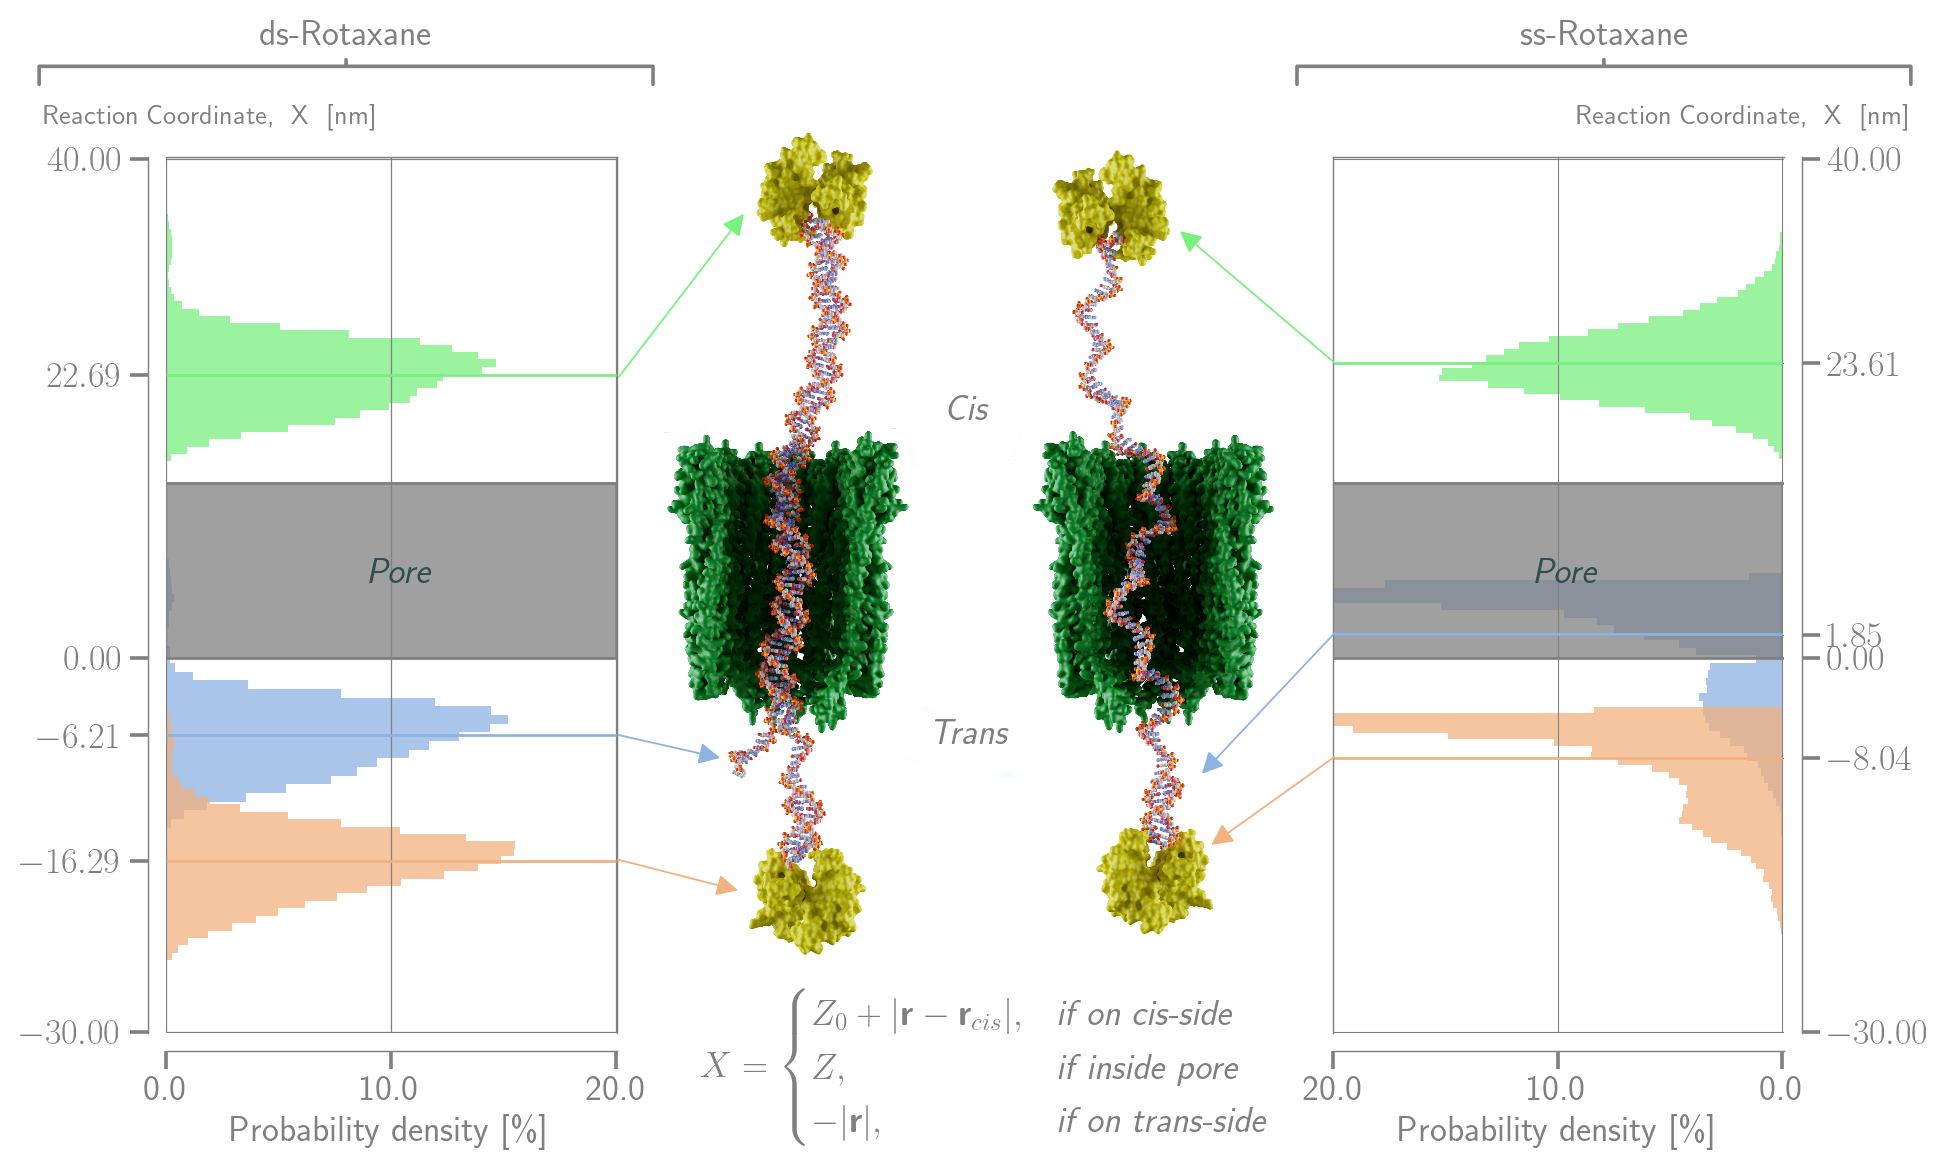
\includegraphics[width=1\textwidth]{Figures/RotaxaneFluctuations.png}
  \caption{write caption}
\end{center}
\end{figure}
